\documentclass{article} % say
\usepackage{tikz}
\usetikzlibrary{calc,arrows,decorations.pathmorphing,backgrounds,fit,positioning}


\begin{document}
%\tikzset{pop1/.style={blue!40},pop2/.style={red!40}}
\centering
    
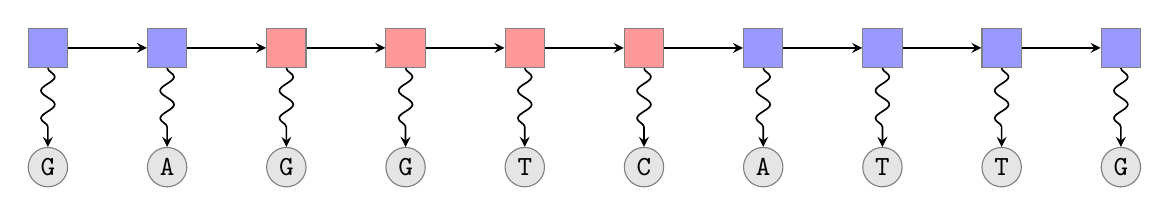
\begin{tikzpicture}[scale=.5]

\tikzset{pop1/.style={fill=blue!40,draw=black!50,inner sep=0pt,minimum size=5mm,shape=rectangle},
pop2/.style={fill=red!40,draw=black!50,inner sep=0pt,minimum size=5mm,shape=rectangle},
allele/.style={fill=black!10,draw=black!50,inner sep=0pt,minimum size=5mm,shape=circle},
transitions/.style={->,>=stealth,semithick},
emissions/.style={->,>=stealth,semithick,decorate,decoration={snake,post length=1mm}}}

% Ancestry states
\node (s1) [pop1] {};
\node (s2) [right=of s1,pop1] {};
\node (s3) [right=of s2,pop2] {};
\node (s4) [right=of s3,pop2] {};
\node (s5) [right=of s4,pop2] {};
\node (s6) [right=of s5,pop2] {};
\node (s7) [right=of s6,pop1] {};
\node (s8) [right=of s7,pop1] {};
\node (s9) [right=of s8,pop1] {};
\node (s10) [right=of s9,pop1] {};

% Emitted alleles
\node (h1) [below=of s1,allele] {\texttt{G}};
\node (h2) [below=of s2,allele] {\texttt{A}};
\node (h3) [below=of s3,allele] {\texttt{G}};
\node (h4) [below=of s4,allele] {\texttt{G}};
\node (h5) [below=of s5,allele] {\texttt{T}};
\node (h6) [below=of s6,allele] {\texttt{C}};
\node (h7) [below=of s7,allele] {\texttt{A}};
\node (h8) [below=of s8,allele] {\texttt{T}};
\node (h9) [below=of s9,allele] {\texttt{T}};
\node (h10) [below=of s10,allele] {\texttt{G}};

% Arrows connecting hidden states
\node (s1.east) {} edge [transitions] (s2);
\node (s2.east) {} edge [transitions] (s3);
\node (s3.east) {} edge [transitions] (s4);
\node (s4.east) {} edge [transitions] (s5);
\node (s5.east) {} edge [transitions] (s6);
\node (s6.east) {} edge [transitions] (s7);
\node (s7.east) {} edge [transitions] (s8);
\node (s8.east) {} edge [transitions] (s9);
\node (s9.east) {} edge [transitions] (s10);

% Arrows connecting states to emissions
\node (s1.south) {} edge [emissions] (h1);
\node (s2.south) {} edge [emissions] (h2);
\node (s3.south) {} edge [emissions] (h3);
\node (s4.south) {} edge [emissions] (h4);
\node (s5.south) {} edge [emissions] (h5);
\node (s6.south) {} edge [emissions] (h6);
\node (s7.south) {} edge [emissions] (h7);
\node (s8.south) {} edge [emissions] (h8);
\node (s9.south) {} edge [emissions] (h9);
\node (s10.south) {} edge [emissions] (h10);

\end{tikzpicture}  

\end{document}